\chapter{Derivation of Parasite Clearance Times}
\section{Introduction}
In the previous progress report submitted in July 2008 the data given to us by GlaxoSmithkline was described and an explanation of how the parasite count is calculated was given. The parasite count is our dependent variable and it was determined that it cannot be treated as a true ``count" for statistical purposes (e.g. Poisson modelling) as it is a value derived from other measurements.

A method for estimating the time to reduce the parasitaemia to 90\% of baseline (PC90) using a cubic fit to the data was presented. These PC90 estimates were then used in 3-way ANOVA, which showed that of the 3 factors \emph{Centre}, \emph{Sex} and \emph{Treatment} that only \emph{Treatment} affected PC90 ($P<0.05$).

This report compares different methods of estimating PC90, such as logistic fitting and linear interpolation, and tries to evaluate which is the best one to use for routine estimation of PC90 for this type of data.
\section{Estimating PC90 for a patient}
\subsection{Cubic regression}
As described in the previous progress report a cubic model was fitted to the log-transformed parasite count $parct$ with time from first dose $t$ as the explanatory variable
$$log(1+parct)=\beta_0+\beta_1t+\beta_2t^2+\beta_3t^3+\epsilon\quad\quad\epsilon\sim N(0,\sigma^2)$$
The data was only fitted up to the first point that parasite count fell to 0 as the subsequent 0 count data is not relevant in determining the time to clearance. PC90 was then estimated from the fit by numerical optimisation with statistical software to find the value of $t$ corresponding to the point where the fitted model crosses a parasite count of $0.1P_0$, where $P_0$ is the initial pre-treatment parasite count.
\subsection{Logistic regression}
The logistic model fitted is
$$log(1+parct)=\alpha+\frac{\lambda}{1+e^{-\beta(t-\mu)}}+\epsilon$$
This was fitted to all the data as it can model a drop from an initial count level to a level of 0, unlike the cubic model. $\alpha$ is the lower asymptote which we would expect to be 0. $\alpha+\lambda$ is the upper asymptote which we would expect to be $P_0$. $\beta$ determines the rate of reduction with time and $\mu$ is the point of inflection (maximum rate of reduction). This model was fitted using non-linear least-squares routines in \emph{R} and \emph{SAS}.
\subsection{Interpolation}
The data points immediately above and below $0.1P_0$ were joined with a straight line fit and then the point where this line crosses $0.1P_0$ determines $t$ at PC90.

For loglinear interpolation the same procedure was performed only on a plot of $log(1+parct)$ vs. $t$.
\section{Comparison of results}
Figures \ref{1MB} and \ref{2FA} compare the logistic with the loglinear interpolation methods; the horizontal line is the PC90 level. It can be seen in Figure \ref{1MB} for Centre 1 male patients on treatment B that there is close agreement between the two methods. However in Figure \ref{2FA} for Centre 2 female patients on treatment A where the data is more ``erratic" that these simple approaches can fail in two ways.

Sometimes the non-linear fitting routine fails to converge on a solution (the plots with no logistic curve). This was found to be a problem using \texttt{nls} in \emph{R}. However, the \texttt{NLIN} routine in \emph{SAS} seems to achieve a reasonable solution in all cases. The second way in which this approach can fail is illustrated in the plot for patient 453 in Figure \ref{2FA} in that the parasite count temporarily dropped below the 10\% level before the actual final elimination of parasites had begun. It is clear that this approach should be modified to identify the \emph{last} time at which the parasite count drops below 10\%.

Table \ref{PC90} shows a comparison of the PC90 estimates by the four different methods looked at so far. Looking at the table the agreement in PC90 estimates looks fairly good. If we perform 6 paired-sample $t$-tests between pairs of methods we find that there is no strong evidence that the cubic regression and linear interpolation methods produce different estimates, likewise for the cubic and loglinear methods and the linear and logistic methods. The other combinations of methods do show evidence of difference in PC90 estimates ($P<0.0002$).

If we repeat the 3-way ANOVA of the previous report we find that \emph{Treatment} is the only factor that affects PC90 whichever method we use. Hence it would seem that the simplest method i.e. linear interpolation is the best method at this stage. However, as we know, the parasite count can be unreliable and depends on an operator-selected ``suitable" blood sample and so just one outlying value could throw the estimate by linear interpolation out as it only uses the two values above and below the PC90 count. In this respect an estimate based on more values should be more robust.
\begin{figure}
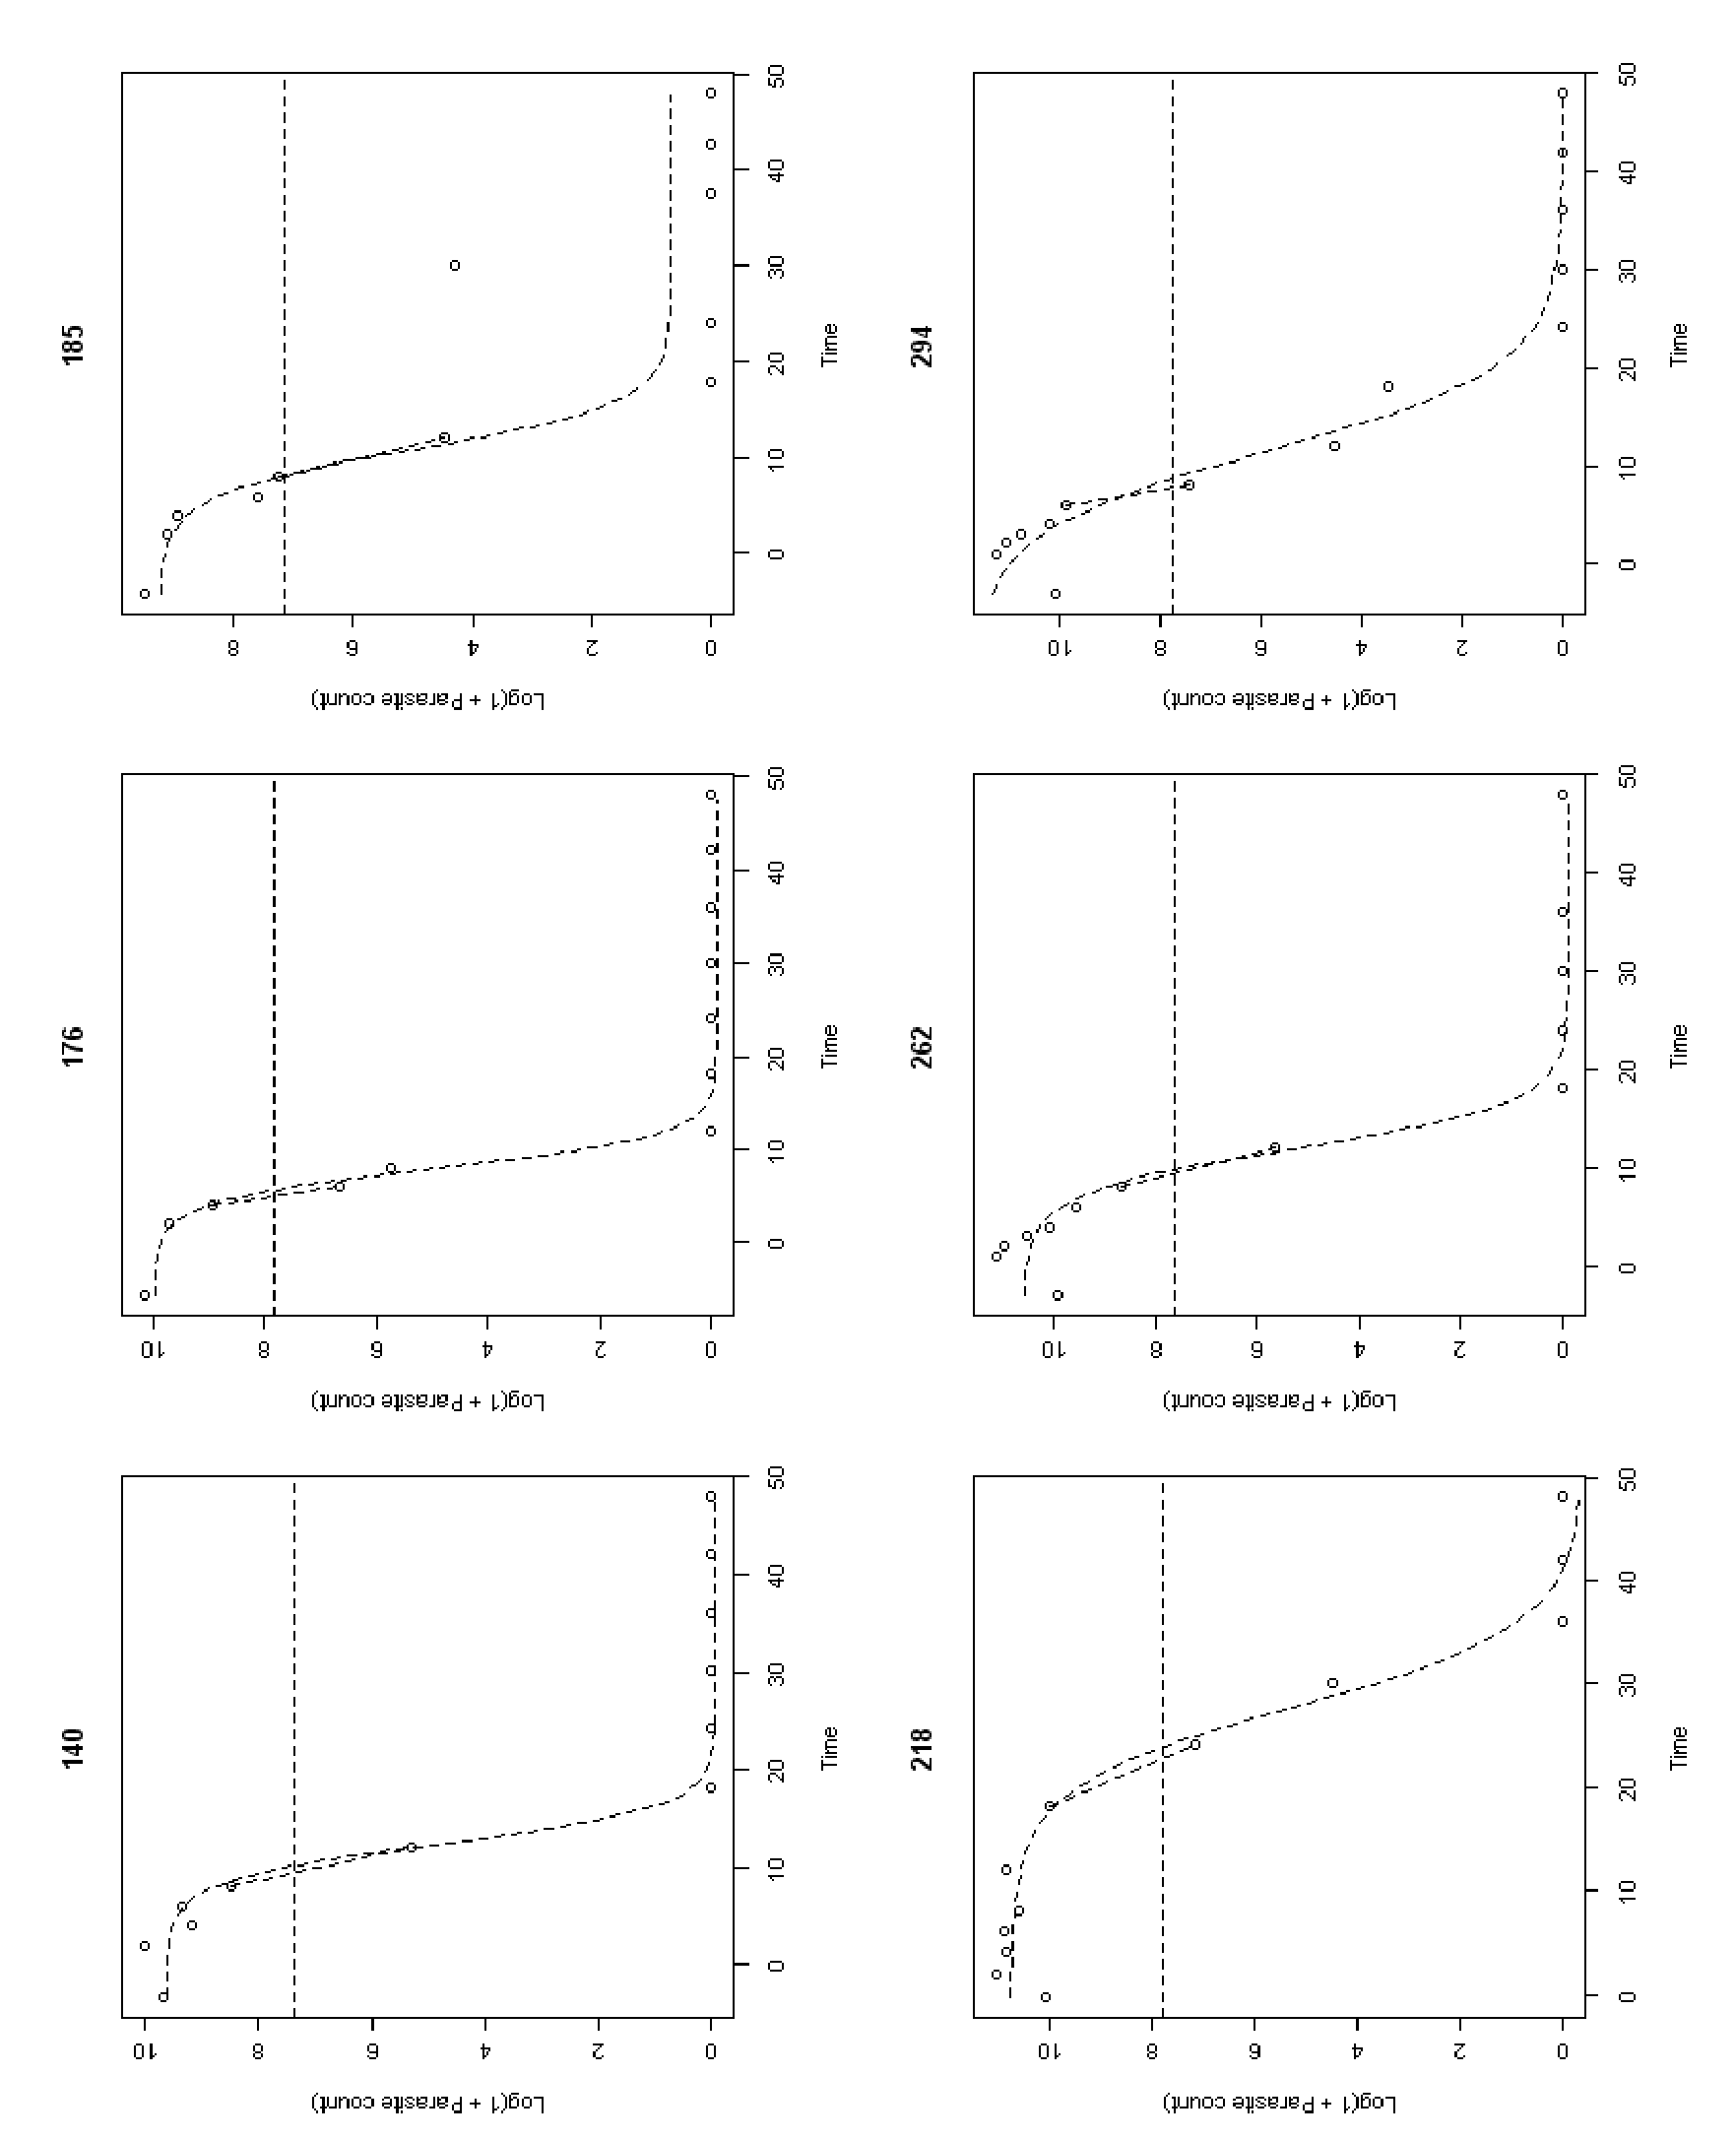
\includegraphics[scale=0.55]{logistic-1MB.eps} 
\caption{PC90 estimates for Centre 1 male patients on treatment B}\label{1MB}
\end{figure}
\begin{figure}
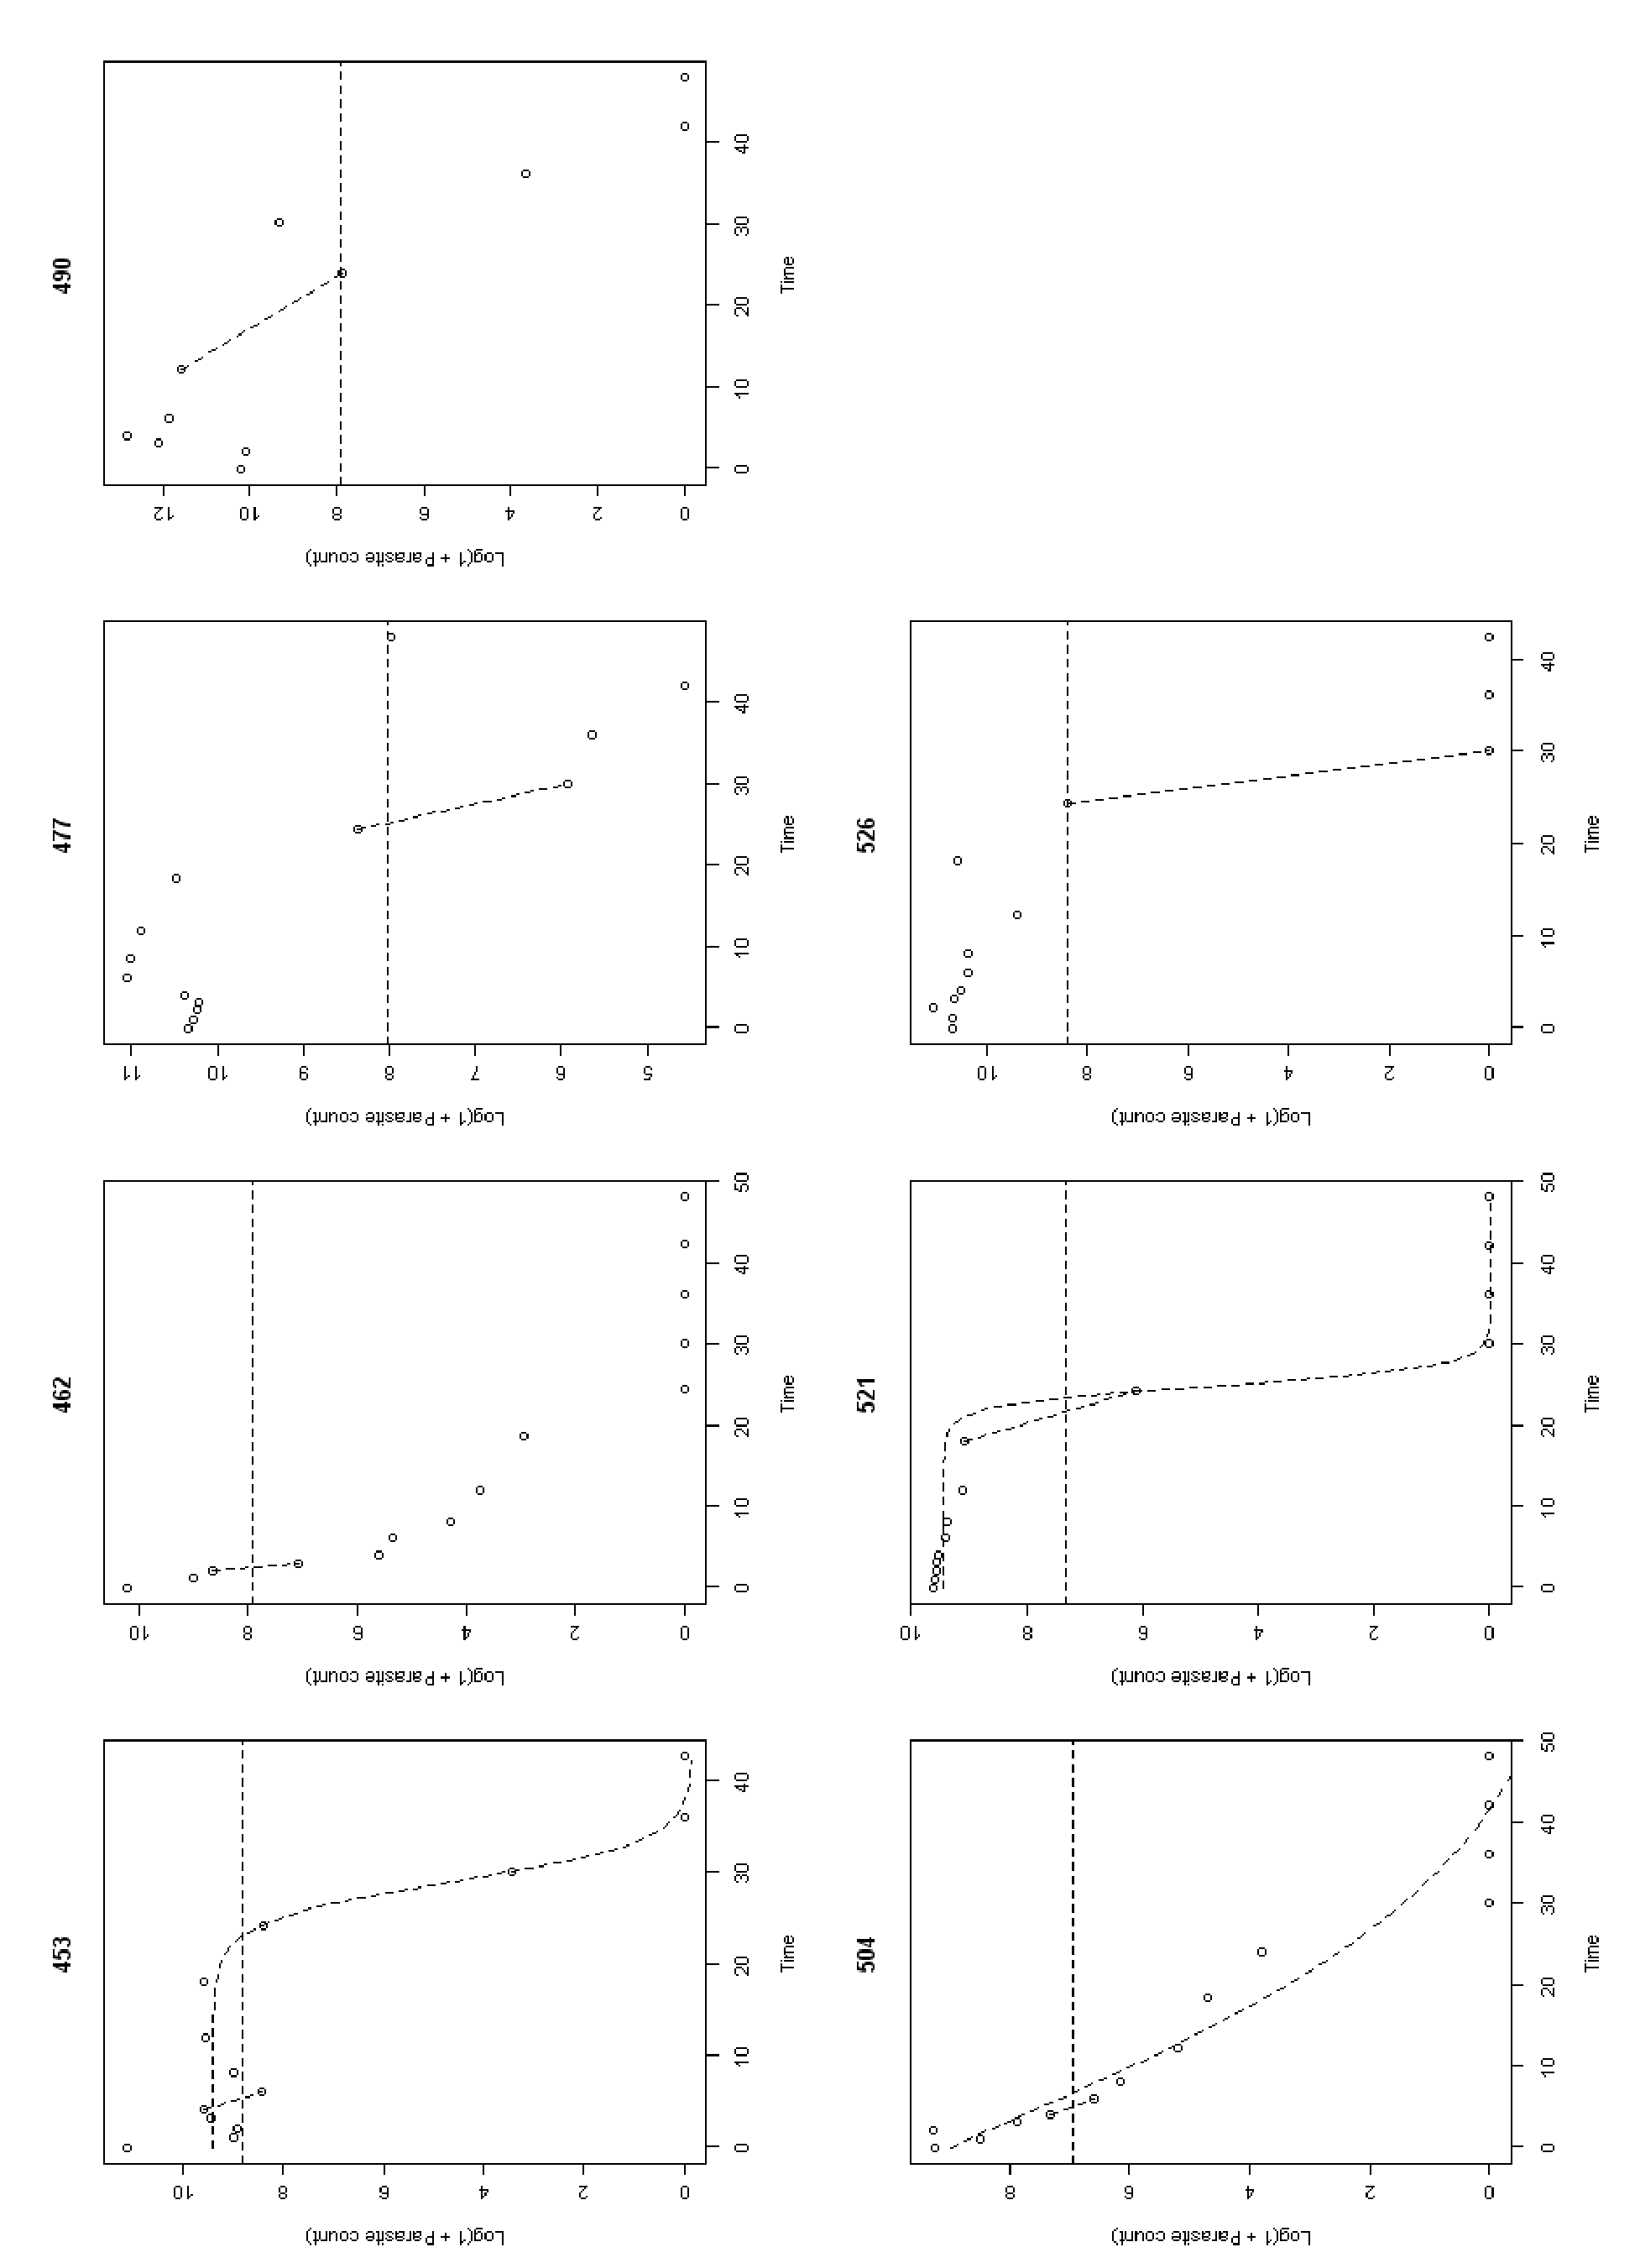
\includegraphics[scale=0.50]{logistic-2FA.eps} 
\caption{PC90 estimates for Centre 2 female patients on treatment A}\label{2FA}
\end{figure}
\begin{table}
\centering
\caption{Comparison of PC90 estimates by 4 methods}\label{PC90}
\begin{tabular}{|cccc|rrrr|}
\hline
Subject&Centre&&&PC90&PC90&PC90&PC90\\
ID&ID&Sex&Treatment&cubic&linear&loglinear&logistic\\
\hline
54&001&M&A&3.82&3.97&3.85&4.14\\
80&001&M&A&27.87&29.73&27.32&28.50\\
96&001&F&A&21.13&20.15&19.76&22.95\\
98&001&M&A&34.25&36.63&36.30&33.51\\
101&001&F&A&23.20&23.87&22.45&\\
140&001&M&B&9.49&10.90&9.46&10.16\\
150&001&F&A&22.53&23.24&21.75&23.12\\
162&001&M&A&9.79&9.10&8.84&\\
176&001&M&B&5.32&5.55&5.05&5.66\\
182&001&F&B&4.18&3.86&3.65&4.29\\
183&001&M&A&4.95&4.50&4.35&\\
185&001&M&B&7.70&8.33&8.09&8.13\\
187&001&M&A&0.83&1.93&1.53&3.05\\
197&001&F&B&8.64&9.87&8.15&8.35\\
203&001&F&B&9.44&11.27&9.69&10.30\\
218&001&M&B&23.54&23.76&22.77&23.92\\
224&001&M&A&28.86&30.02&30.01&30.26\\
262&001&M&B&9.40&10.74&9.40&9.85\\
264&001&F&B&0.88&0.96&0.85&1.43\\
280&001&F&B&8.61&9.92&9.04&9.72\\
285&001&F&A&47.24&46.76&46.52&\\
288&001&F&B&12.86&9.67&9.38&12.38\\
294&001&M&B&8.11&7.93&7.73&8.68\\
295&001&M&A&4.67&5.11&4.83&4.98\\
449&002&M&A&4.50&5.42&4.82&\\
453&002&F&A&20.07&22.73&21.97&23.08\\
462&002&F&A&2.22&2.67&2.49&\\
469&002&M&A&2.15&2.26&2.21&\\
477&002&F&A&24.03&26.10&25.08&\\
490&002&F&A&28.73&24.10&24.17&29.94\\
500&002&M&B&19.35&18.03&17.15&19.66\\
502&002&F&B&15.39&16.10&14.77&16.33\\
504&002&F&A&5.04&5.18&5.00&6.64\\
505&002&F&B&8.37&10.30&8.74&9.02\\
509&002&M&A&20.58&11.79&11.59&18.63\\
511&002&M&B&9.99&10.55&9.51&10.91\\
519&002&M&B&15.60&16.54&14.68&16.08\\
521&002&F&A&22.21&23.34&21.64&23.38\\
523&002&F&B&5.90&5.93&5.84&7.20\\
525&002&F&B&6.26&6.91&6.11&6.17\\
526&002&F&A&23.71&24.46&24.42&\\
530&002&M&A&29.07&29.53&28.09&29.28\\
532&002&M&B&8.94&8.33&8.08&9.21\\
\hline
\end{tabular}
\end{table}
\section{Ongoing work plan}
\begin{itemize}
\item Look at ways to pick sensible starting values for the logistic regression and check that the logistic form is valid.
\item Investigate the effects of outliers on the estimation of PC90 and determine how to detect and deal with them.
\item Incorporate the uncertainty in PC90 estimates into the modelling of treatment effect. 
\item Compare parametric and non-parametric approaches to determining which factors affect PC90.
\item Look at non-parametric inference for determining confidence of PC90 estimates e.g. randomisation.
\end{itemize}